  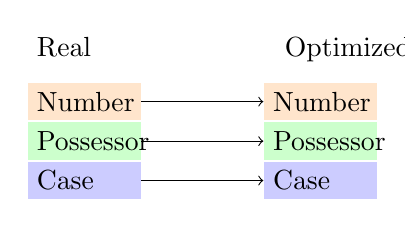
\begin{tikzpicture}[%
% common options for blocks:
block/.style = {draw, fill=blue!30, align=center, anchor=west,
            minimum height=0.65cm, inner sep=0},
% common options for the circles:
ball/.style = {circle, draw, align=center, anchor=north, inner sep=0}]
\node[rectangle,text width=1.2cm,anchor=base] (A0) at (1,-0.3) {Real};
\node[rectangle,text width=0.9cm,anchor=base] (B0) at (4,-0.3) {Optimized};
\node[rectangle,text width=1.2cm,anchor=base, fill=orange!20] (A1) at (1,-1.0) {Number};
\node[rectangle,text width=1.2cm,anchor=base, fill=green!20] (A2) at (1,-1.5) {Possessor};
\node[rectangle,text width=1.2cm,anchor=base, fill=blue!20] (A3) at (1,-2.0) {Case};
\node[rectangle,text width=1.2cm,anchor=base, fill=orange!20] (B1) at (4,-1.0) {Number};
\node[rectangle,text width=1.2cm,anchor=base, fill=green!20] (B2) at (4,-1.5) {Possessor};
\node[rectangle,text width=1.2cm,anchor=base, fill=blue!20] (B3) at (4,-2.0) {Case};
\draw[->] (A1.east) to (B1.west);
\draw[->] (A2.east) to (B2.west);
\draw[->] (A3.east) to (B3.west);
\end{tikzpicture}
